\documentclass[11pt,parskip,abstracton,notitlepage, paper=a4]{scrartcl}

\usepackage{amssymb, amsmath, amsthm, graphics, graphicx, longtable, setspace, makeidx, subfig, marvosym, microtype, booktabs, authblk, lipsum, siunitx, lscape}

\usepackage{lmodern}
\usepackage[T1]{fontenc}
\usepackage[utf8]{inputenx}% For proper input encoding
\usepackage[margin=10pt,font=small,labelfont=bf,labelsep=endash]{caption}
\KOMAoptions{DIV=last}

\usepackage[style=authoryear,natbib=true, 
url=false,
isbn=false,
doi=false,
bibencoding=utf8,
maxbibnames=10, 
maxcitenames = 2, 
mincitenames = 1, 
firstinits = true,
uniquename=false, 
uniquelist=false,
useprefix=true,
backend=biber]{biblatex}
\renewcommand*{\compcitedelim}{\addsemicolon\space}
\renewbibmacro{in:}{}
\setlength\bibhang{20pt}
\bibliography{references}
\AtEveryBibitem{%
	\clearfield{day}%
	\clearfield{month}%
	\clearfield{endday}%
	\clearfield{endmonth}%
}
\doublespacing
%\onehalfspacing
\KOMAoptions{DIV=last}
\usepackage[pdftex,colorlinks=true,citecolor=magenta,urlcolor=magenta,pdfstartview=FitH]{hyperref}
\pdfcompresslevel=9
\hypersetup{pdftitle=Regional competition and place-based economic growth: Determinants of competitiveness, pdfauthor={Thomas de Graaff, Frank G. van Oort, Mark Thissen}}


\begin{document}
	
	\title{Regional competition and place-based economic growth: Determinants of competitiveness\thanks{The authors would like to thanks participants of the Eureka seminar at the Vrije Universiteit Amsterdam and of the NECTAR conference in Ann Arbor for useful comments and suggestions. The usual disclaimer applies.}}
		\author[1]{\normalsize Mark Thissen}
		\author[2]{\normalsize Thomas de Graaff\thanks{Corresponding author: Thomas de Graaff. Email: \url{t.de.graaff@vu.nl}}}
		\author[3]{\normalsize Frank G. van Oort}
		\affil[1]{\normalsize PBL Netherlands Environmental Assessment Agency}
		\affil[2]{\normalsize Department of Spatial Economics, VU University Amsterdam, the Netherlands}
		\affil[3]{\normalsize Erasmus University Rotterdam, The Netherlands}
		\date{\normalsize\today}
		\maketitle
		\clearpage
		\begin{abstract}
			\noindent
				Regional economic growth is equivalent with a region producing and selling more or better products and services which can be due to an increase in demand from other regions, or can be due to a change in regional characteristics raising productivity and the competitive position of the region itself. Most of the existing spatial econometrics literature is about the measurement of these regional characteristics that can be spatially correlated via regional spillovers. In this paper, instead, we focus on the influence of the relative score of a region's characteristics vis-\`{a}-vis their competitors on a region's economic growth performance.
				
				We do so by decomposing regional value added growth in two parts: a part that is demand induced due to growth in the region's export markets and a part that is due to changes in market shares in the region's export markets. This last component of economic growth (coined structural growth) is hypothesized to be affected by different characteristics of competing regions. To compare the economic performance of these regional competitors we therefore estimate a regional growth regression using geographical weighted regression, where the weights in the geographical weighted regression are the degree of competition between sectors from different regions. 
				
				The result show that region specific characteristics are only important in specific (geographical) markets. This has important policy implications since it emphasizes the importance of recently advocated place based policies. 
				 \\
			\newline
			{\small \textbf{Keywords: Structural regional growth, competition networks, demand-led regional growth, geographically weighted regressions}}\\
			{\small JEL classification: R11, R15, R58.}
		\end{abstract}
		\clearpage
\section{Introduction}

The concept of regional competitiveness is a dominant concept in public policy \citep{Bristow2005} and increasing competitiveness is an explicit policy goal by regional, national and supra-national governments (i.e. the European Commission) across Europe \citep{baldwin2009european}. Relevant regional policies involve the conditions under which economic activities can prosper \citep{Bristow2010}. An increasing competitiveness strategy involves the ability of regional governments to learn about the effects of economic policy, particularly through methods based on comparison or monitoring. Henceforth, benchmarking and regional econometrics have become particularly popular within regional economic policy-making in recent years \citep{huggins2010regional} as they measure and compare competitive regional performance \citep{beaudry2009s,DeGroot2009a,melo2009meta}. 

Conceptually, regional benchmarking and regional econometrics has progressed from quite simplistic forms that compare and rank different regions to more complex modes \citep[see][p. 642, with respect to benchmarking]{huggins2010regional}. The main critique on the simplistic approaches highlighted the distinctiveness of regional environments as limiting the utility of what is considered ‘copy-and-paste’ and ‘one-size-fits-all’ policy-making, as regional stakeholders purport to transfer perceived ‘best practices’ from one region to another \citep{huggins2010regional}. Concerning regional development, \citet{malecki2002hard} and \citet{tracey2003alliances} have therefore drawn attention to the potential importance of interregional and international networks as sources of goods and knowledge in shaping firm competitiveness in a particular area. In particular, spatial econometrics and the concept of revealed competition \citep{thissen2013regional} bring interregional relatedness, region specific markets and circumstances into the econometric and benchmark evaluation of regional economic performance. 

In spatial econometrics the focus has been on measuring regional characteristics to capture the effect of regional spillovers on economic growth. This extensive body of literature showed that there is strong spatial autocorrelation over short distances that can be either caused by these regional spillovers or due to strong demand effects from neighbouring regions. [UITBREIDEN: FRANK?]. \citep[see, e.g.,][]{dall2003regional, le2006evaluating, le2008spatial}

Regional economic growth in itself is equivalent with a region producing and selling more or better products and services. Regional economic growth can have two distinct sources. It can be due to economic growth and the corresponding demand from other regions (from here on denoted as demand-led growth), or it can be due to regional characteristics raising productivity (from here on denoted as structural growth). If we represent the total economy as a large pie the first source of regional economic growth is due to growth of the total pie, while the second source is due to a region gaining a larger share of the pie. The first source of regional growth cannot be influenced by the region's governments as it is due to the independent growth of a region's export destinations. The second source of regional growth is due to structural characteristics inducing an increase in market shares and thereby the result of an increase in a region's competitiveness.

In accordance with this division of regional economic growth in a demand-led and a structural component we can distinguish three different channels via which regional characteristics may affect regional economic growth: 
\begin{enumerate}
	\item The growth of a region may be influenced by the regional characteristics of neighboring regions via demand-led growth effects. This is a trickledown effect from growing regions towards supplying regions.
	\item A region specific characteristics may affect the competitiveness of regions increasing the market share of firms in that region at the expense of its competitors from other regions. 
	\item Other regions' characteristics may spillover to neighboring regions. The quintessential example of this effect are agglomeration effects where smaller regions may profit from the success of their larger neighbors.
\end{enumerate}

In this paper we will focus on the second channel; so, how may regional characteristics affect regional economic growth via a gain in this region's market share. The first and third channel is extensively discussed in the spatial econometrics and regional trade literature. 

Importantly, regional characteristics can be influenced by the region itself which gives it an instrument to influence its competitiveness. Demand-led growth (or decline) is in general beyond a region's sphere of influence. In other words, a region may perform excellent locally but go into recession because of a lack in demand from other regions. Vice versa it may be the case that a region under-performs but still grows due to external characteristics. In this last case a region would under-perform relative to its potential. Obviously, this leads to important implications for benchmarking and econometric analysis alike: typically, only structural growth can be affected by regional policies and should therefore be taken into account in a policy evaluation.

Although structural growth is of primal importance to evaluate regional policy, demand led growth may be the most important factor explaining regional economic growth. Economic connections with growing markets and crucial trade hubs, can strongly affect growth opportunities as it determines the degree to which regional development is connected to growth conditions in other regions. The economic crisis in Europe that started with the banking crisis in 2008 and to some degree still continues into 2015 is characterized by such interregional spillovers of (negative) growth. These negative growth spillovers explain a large part of regional economic development, but make it difficult to analyze the performance of regions and thereby the effectiveness of regional policies to enhance a region's competitiveness. A region may implement excellent regional policies and relatively outperform many other regions while having a negative growth rate. This negative growth rate may be caused by a collapse in the demand for goods and services from other regions. We therefore have to take a closer look at regional economic growth. More specifically, we have to distinguish between regional growth that is the result of an increase in demand in other parts of the world, and growth that is due to a change in structural characteristics strengthening a region's competitiveness and increasing its productivity. 

In this paper we therefore decompose growth in structural and demand led regional growth components using interregional trade data and supply and use information. The growth decomposition offers therefore an innovative perspective on distinguishing regional characteristics determining development opportunities that can be influenced by regional policy makers, from international economic network determinants that is much less easy to plan locally. Insight in this local-global blend of influences is important for distinguishing competitive strength and opportunities, and, related to that, location characteristics that locally can make a difference and may be subject to policy attention. 

We also determined the revealed competition \citep{thissen2013regional} to measure the degree of competition between firms from different regions. This degree of competition matrix gives us the region specific weights in which differences in regional characteristics may affect regional economic growth by gaining market share at the expense of competitors from different regions. For our regional growth regressions, we use a geographical weighted regression specification to take all these different region-specific market areas into account.

Our econometric analysis shows the strong place-based foundation of regional competitiveness and gives thereby an important contribution to the ongoing policy debate on place-based or place-neutral development strategies in the European Union. This debate is highlighted in the context of a series of recent major policy reports: the place-neutral policies in the 2009 World Bank report \citep{worldbank2009} and the European place-based development strategies in \citet{barca2009agenda} and \citet{barca2012case}. 

The paper is structured as follows. The next section discusses in detail the concepts of competitiveness and revealed competition and explains very carefully how we construct our structural and demand-led growth measures. Section \ref{sec:data} given an overview of the data we use. Section \ref{sec:model} spells out in detail the economic and econometric we employ, whereafter section \ref{sec:results} discusses the results. The last section concludes. 

\section{Competitiveness, revealed competition and economic growth}

By tradition, economists argue that competition is good, as it brings out the best of firms and regions and will ensure an efficient distribution of investments \citep{glaeser2001economics}. Measurement of competition and the various sources of growth is however difficult. Economic growth is in general equivalent to producing and selling more products and services. As argued before, this economic growth can have two distinct sources. It can be due to economic growth and demand from other regions, or it can be due to internal characteristics raising productivity. 

Conventionally the international trade literature has focused on variants of revealed comparative advantage (RCA) as presented by the \citet{balassa1965trade} Index. In the Balassa index the shares of different product categories in total exports of a country are compared to the shares of a group of reference countries. The Balassa index determines what types of products are overrepresented in a country's exports and tells us what export products a country is relatively ``good'' in. The competition between two regions is commonly measured by comparing the export structure of two regions in a specific market using \citet{finger1979measure} export similarity index. Analogous to the Balassa index it measures to what degree two regions have the same comparative advantage in a specific regional market. The principle of revealed competition \citep{thissen2013regional} between regions concerns their market overlap. The competition a region $A$ receives from a region $B$ depends on two characteristics. First, it depends on the market share of firms from region $ B $ in each region. Secondly, it depends on the importance of each of the markets for region $ A $, where a market is important for region $ A $ if a substantial share of its sales is destined to it.  Accordingly, region $ A $ receives strong competition from region $ B $ if region $ B $ has a large market share in the regions which are important for region $ A $. The competition between regions $ A $ and $ B $ would be less strong if region $ B $ has a large market share in the regions which are unimportant for region $ A $, or if region $ B $ would have a low market share in the regions which are important for region $ A $. After all, in such situations, there is only a limited market overlap and firms from regions $ A $ and $ B $ would have fewer opportunities to take market shares from each other. By investigating the market overlap, we obtain insight into the markets being most important for firms and the regions from which they obtain strongest competition.

The growth decomposition introduced in this paper places the concept of revealed competition in a dynamic context analyzing the developments in a region's market area. The growth decomposition can be easily explained by representing the total economy as a large pie. The first source of regional economic growth is due to growth of the total pie, while the second source is due to a region gaining a larger share of the pie. The first source of regional growth cannot be influenced by the region's governments as it is due to the independent growth of a region's export destinations. The second source of regional growth is due to structural characteristics inducing an increase in market shares and thereby the result of an increase in a region's competitiveness. These structural characteristics can be influenced by the region itself. Demand induced growth (or decline) is beyond a region's sphere of influence.

In the subsequent two subsections we will define both revealed competition as well as the growth decomposition in more detail.

\subsection{Revealed competition}

[HIER AANVULLEN: OP BASIS VAN SECTOREN EN REKENING HOUDEND MET SAMENSTELLINGSEFFECTEN]

\subsection{Value added regional growth decomposition}

In order to explain the decomposition of regional economic growth in demand led and structural growth more formally we first define the market share $M_{p,i,j,t}$  in products $p$ of (producing) region $i$ in (market) region $j$ during time period $t$ as described in the following equation:

\begin{equation}
M_{i,j,t} = \frac{H_{p,i,j,t}}{D_{p,j,t}},
\label{eq:Mijt}
\end{equation}

where $H_{p,i,j,t}$  is the trade from region $i$ to region $j$ and $D_{p,j,t} = \sum_i{H_{p,i,j,t}}$  is the demand or size of the market in region $j$. Please note that the regions are used to describe both producing regions as the markets or regions where the products are sold.

We can now define the two different growth components. The demand led growth $G_{p,i,t}^{dem,x}$  measured in production levels $x$  is equal to:

\begin{equation}
G_{p,i,t}^{dem,x} = \sum_j {M_{p,i,j,t} \left(D_{p,i,j,t} - D_{p,i,j,t-1} \right) }
\label{eq:Gdem}
\end{equation}

and the structural growth $G_{p,i,t}^{struc,x}$ is therefore defined as:

\begin{equation}
G_{p,i,t}^{struc,x} = \sum_j {\left(M_{p,i,j,t} - M_{p,i,j,t-1} \right)D_{p,i,j,t} },
\label{eq:struc}
\end{equation}

such that the overall absolute growth $G_{p,i,t}^{x}$ is equal to the sum of both the demand led $G_{p,i,t}^{dem,x}$ and the structural growth $G_{p,i,t}^{struc,x}$.

However, the growth of production may be the result of an increase in the price of intermediate goods and thereby production costs. As a consequence the growth in the value of production may not be representative for the actual absolute growth of regional GDP. It is therefore important to calculate the associated value added with the increase in these production levels. A complicating factor to translate the production value into value added is that value added is used in the production process to produce different products. We therefore have to use information from both the supply and the use tables to correctly translate the growth in production value into the growth in value added.

The formula's for the growth decomposition in value added are therefore as follows. The demand led growth $G_{p,i,t}^{dem,va}$ measured in value added $va$ is equal to:

\begin{equation}
G_{p,i,t}^{dem,va} = \sum_s V_{s,i,t}T_{s,p,i,t}{\sum_j {M_{p,i,j,t} \left(D_{p,i,j,t} - D_{p,i,j,t-1} \right) }}
\label{eq:Gdemva}
\end{equation}

and the structural growth $G_{p,i,t}^{struc,va}$ in value added is therefore defined as:

\begin{equation}
G_{p,i,t}^{struc,va} = \sum_s V_{s,i,t}T_{s,p,i,t}{\sum_j {\left(M_{p,i,j,t} - M_{p,i,j,t-1} \right)D_{p,i,j,t} }},
\label{eq:strucva}
\end{equation}

Where $V_{s,i,t}$ can be directly taken from the regional use table and is the value added used per unit production of sector $s$ in region $i$, and $T_{s,p,i,t}$ can be directly taken from the regional supply table and is the technology parameter that gives the share of products $p$ produced per unit production of sector $s$ in region $i$. Notice that the overall absolute growth in value added also equals the sum of both the demand led and the structural growth.

\section{Data\label{sec:data}}

[MARK EN FRANK NOG AANVULLEN; SPECIFIEKER, DE BRONNEN VAN SUPPLY AND USE TABLES TOGETHER WITH THE FACTOR REWARDS AND THE REGIONAL CHARACTERISTICS; LET OOK OP: WE GEBRUIKEN NU DE PERIODE 2000-2007]

This paper introduces a value added growth decomposition method based on an analyses of trade between European regions and the market shares on European regional markets. This method is implemented on the PBL multiregional Supply and Use tables \citep{Thissen2013b, Thissen2013} and gives region specific sources of economic growth. 

\begin{figure}
	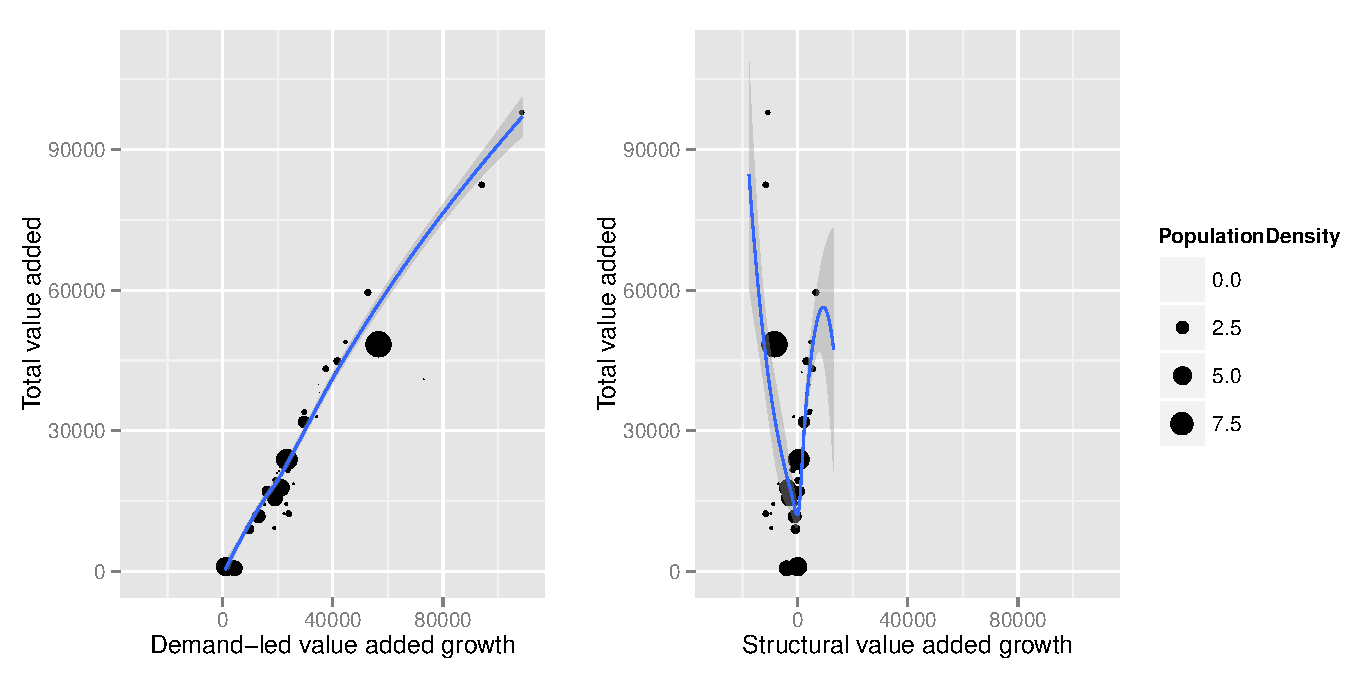
\includegraphics[width=1\textwidth]{../Fig/Decomposition}
	\caption{Decomposition of European Regional Growth}
	\label{fig:decomposition}
\end{figure}

Figure \ref{fig:decomposition} shows the decomposition of total growth in structural growth and demand-led growth for our sample at a similar scale. Clearly, we can see that (\textit{i}) total value added growth is almost perfectly correlated by demand-led value added growth and (\textit{ii}) demand-led growth dominates structural value added growth in terms of size. So, regional economic performance is mostly governed by a proces regional polic makers cannot influence---or only to a very limited extent. 

\begin{figure}
	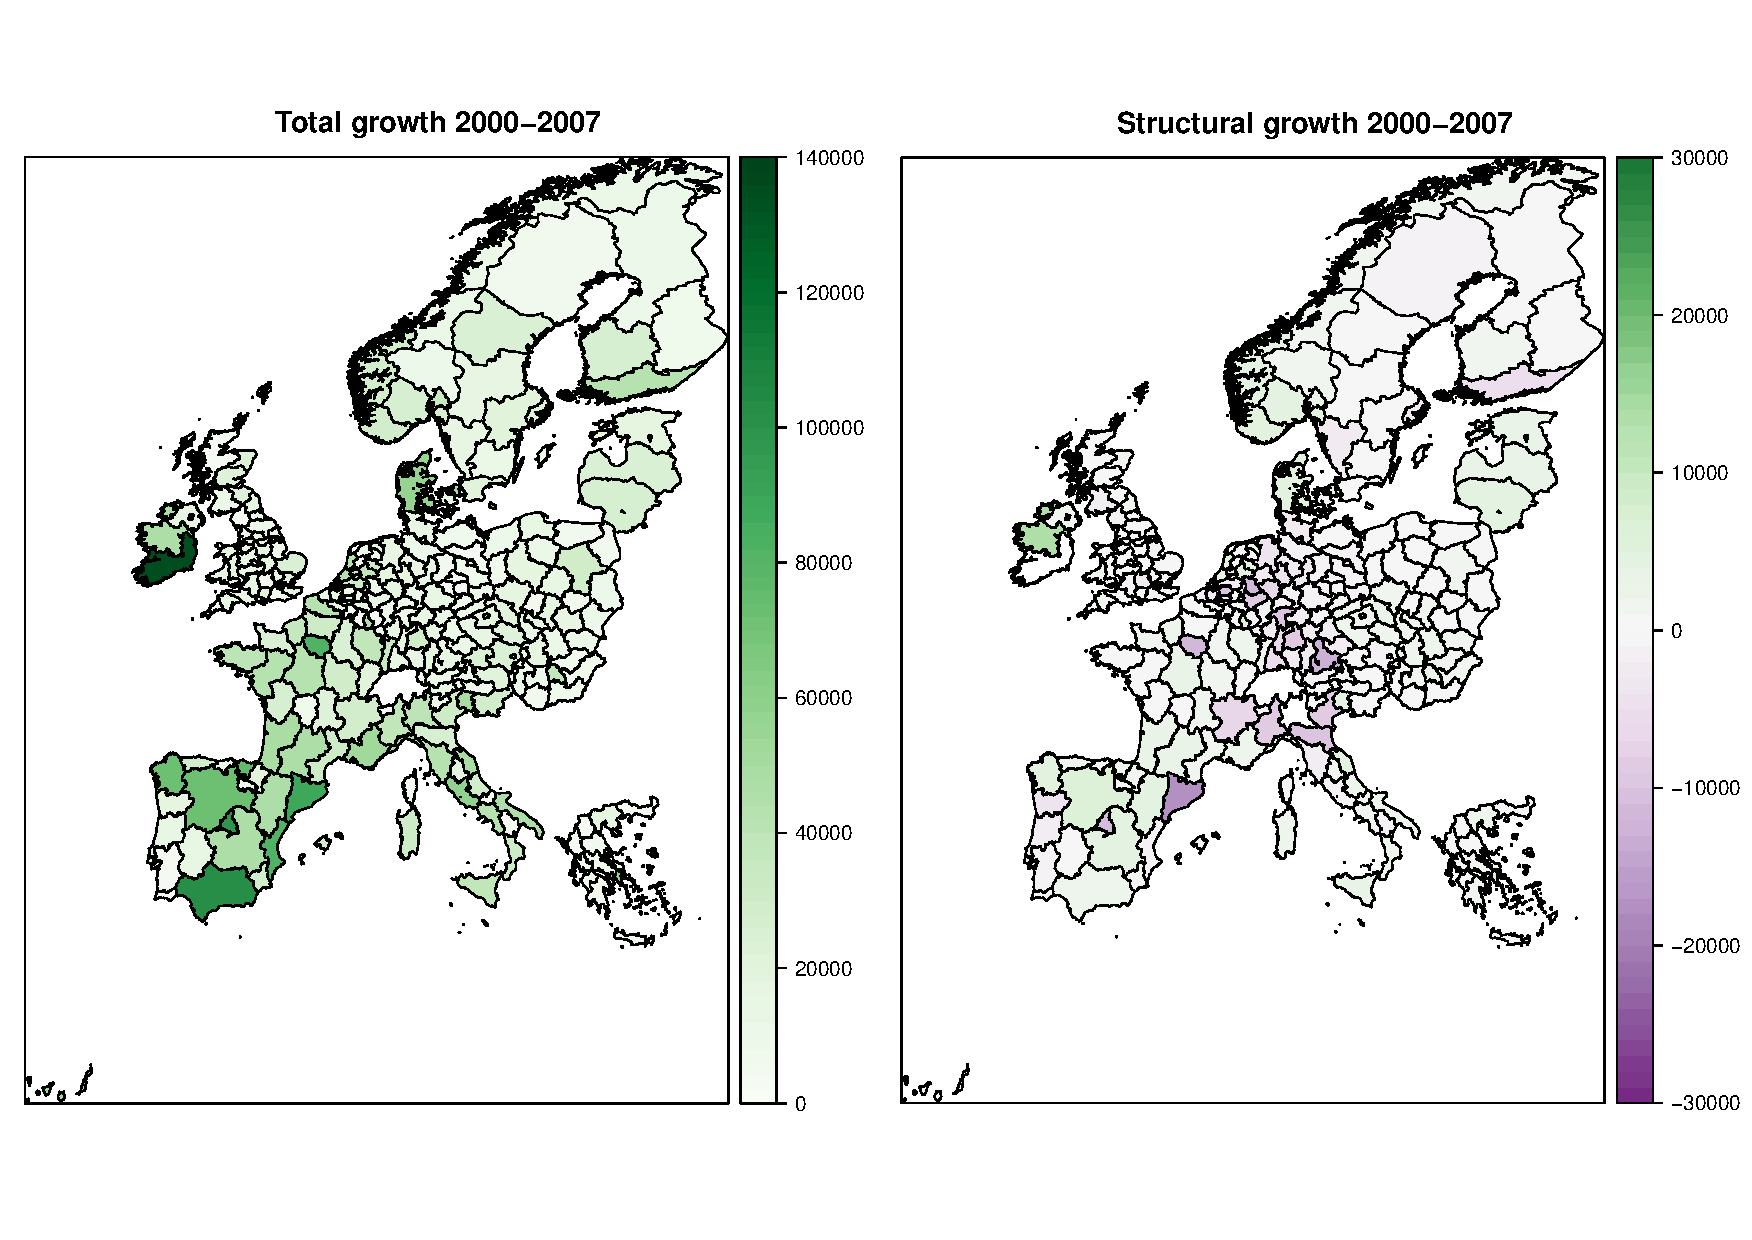
\includegraphics[width=1\textwidth]{../Fig/VAGrowth}
	\caption{Total and structural growth across European Regions in the period 2000-2007}
	\label{fig:mapsgrowth}
\end{figure}

The regional variation of value added and structural value added growth can be seen in Figure \ref{fig:mapsgrowth}. Clearly, all European regions experienced value added growth in the period 2000-2007, and especially the regions in the periphery of Europe indicating large catching-up effects. However, most of the growth is governed by demand-led growth. So, structural value added growth is even found to be negative for especially the European core regions, most notably in Germany and Northern-Italy.

\section{Modeling the effect of competitiveness on regional economic growth\label{sec:model}}

To understand which determinants affect structural growth and how revealed competition affect the effectiveness of these determinants, we adopt two different strands of literature. For our baseline regression approach, we adopt the well know neoclassical Solow-Swan growth model \citep{MANKIW1992} and apply it to the regional case \citep[conform, e.g.,][]{ABREU2005}. Secondly, we adopt a non-parametric 'geographically' weighted regression approach \citep{brunsdon1998geographically} for our specification, where we allow our coefficients to vary over the revealed competition network instead of over space. The latter gives insight into what extent determinants have a place-based or place-neutral impact on regional performance.  

\subsection{The neoclassical regional growth model}

To model regional economic growth, we estimate the following linear regional growth model:
\begin{equation}
	\ln\left(\frac{y_{r,s,2007}}{y_{r,s,2000}}\right)=\beta_c+\beta_1\ln(y_{r,s,2000}) + \beta_2 \ln(i_{r,s, 2000}) + \beta_3 \ln(n_{r,s, 2000}) + \ln{\mathbf{X}_{r, 2000}} \beta_4,
	\label{regionalgrowth}
\end{equation}
where $y_{i,s,t}$ is structural value added in region $r$, sector $s$ at time $t$, per worker working in that sector, $\nu_c$ denotes a constant which we allow to vary over country, $i_{s,1000}$ is the regional investment rate in sector $s$ in the year 2000, $n_{r,s,2000}$ the regional worker growth rate in sector $s$ in the year 2000 and $\mathbf{X}_{r,2000}$ are regional determinants measured in the year 2000 that might influence regional performance and thus may serve as policy instruments. Finally, the $\beta$'s are (vectors of) parameters that we want to estimate. 

Note that the left-hand side composes a growth rate, that $\beta_1$ accounts for regional catching up effects, and that instead of a regional savings rate, we adopt a regional investment rate as the latter has a more straightforward interpretation in a regional growth context.\footnote{Typically, regional consumption does not match regional investments. A good example would be the European Regional Development Funds that serve as regional investments.}. Moreover, theoretically, $n$ encompasses as well autonomous technological growth and a depreciation factor. Because these two do not vary over regions and are usually unknown we proxy these two---as commonly done---with a generic growth percentage of 6\% per year. Theoretically, the inequalities $\beta_1, \beta_3 <0$ and $\beta_2  > 0$ should hold.  

The supply and use tables as discussed in section \ref{sec:data} provides us as well with the factor rewards for both labor and capital. This allows us to deal with one of the prevailing data problems in this literature: the calculation of the capital stock. Typically this is done with a perpetual inventory method. However, this could be problematic, since shocks in the capital stocks (e.g, by deaths or migrations of a firms) do not manifest themselves in the short run. Because we have information on  regional value added of capital ($V^K$) across regions, sectors and years (so $V^K_{r,s,t} = r_{r,s,t} K_{r,s,t}$), we can circumvent this problem by using data on sector specific interest rates for capital and thus calculate the capital stock per region, year and sector ($K_{r,s,t}$).\footnote{Unfortunately but not surprising, we only have country specific interest rates instead of region specific.}

This allows us to calculate the sectoral and regional investment rates calculated from the capital growth equation as typically used in the neo-classical growth model:
\begin{equation}
\Delta K_{r,s,t} = i_{r,s,t} Y_{r,s,t} - \delta K_{r,s,t}
\label{eq:capitalgrowth}
\end{equation}
Equation (\ref{eq:capitalgrowth}) allows us to tease out the regional investment rates ($i_{r,s,t}$) as a result from the supply and use tables and to estimate the regional growth model in equation (\ref{regionalgrowth}).

\subsection{The `geographically' weighted model of structural regional economic growth}

Estimating (\ref{regionalgrowth}) by OLS allows us to assess the \textit{average} size of the $\beta$ parameters across all regions. However, if policy instruments do not possess a `one size fits all' character, then we should allow for parameter heterogeneity. We therefore resort to geographically weighted regressions (GWR). 

Originally, GWR is an exploratory technique mainly intended to indicate where non-stationarity is taking place on the map \citep{bivand2014package}. It allows coefficients and thus their marginal effects to change via a predefined metric (which is typically Euclidean distance). Basically, it is a non-parametric technique and can in a regression framework be described as \citep[see for more details][]{fotheringham2003geographically}:
\begin{equation}
y_i = \beta_0(u_i, v_i) + \sum_k (\beta_k) (u_i, v_i) \mathbf{X}_{ik} + \epsilon_i
\label{eq:GWR}
\end{equation}
where $y$ denotes the endogeneous variables, $X$ a matrix of exogeneous variables and $\beta$ a coefficient vector. The only difference with a global regression approach is that $\beta$ is now allowed to vary over a predefined metric or network where $u_i$ and $v_i$ typically stand for region's $i$ longitude and latitude, respectively. 

Essentially, Eucledian distance is not required as long as one uses a predefined metric for each region. This finally results in a $n \times n$ matrix, $\mathbf{W}(i)$, whose off-diagonal elements are zero and whose diagonal elements (denoted by $w_{ij}$) constitute a weighting defined by the metric for each of the regions for regression point $i$. Or, in mathematical notation \citep[\textit{cf}.][]{fotheringham2003geographically}:

\begin{equation}
\mathbf{\hat{\beta}}(i) = \mathbf{X'W}(i)\mathbf{X^{-1}X'W}(i)y
	\label{eq:coefficient}
\end{equation}

This results in a weighted least squares estimator where the weights vary for each region $i$. Note that the weighted regression (\ref{eq:coefficient}) varies for each region $i$. We adopt for the weighting scheme $\mathbf{W}(i)$ a gaussian kernel, denoted as:

\begin{equation}
	w_{ij} = \exp\left[-\left(\frac{d_{ij}}{2b}\right)^2\right],
	\label{eq:weights}
\end{equation}
where $b$ refers to the bandwidth, which we first have to optimize by a cross-validation procedure \citep[for more information we refer to][]{fotheringham2003geographically}.

\section{Results\label{sec:results}}

We first present the estimation results for the neoclassical growth model, after which we show that---by using geographically weighted regressions implemented by revealed competition networks---the parameters vary systematically over regions and that using revealed competition networks perform slight better than using an Eucledian distance metric in explaining European regional economic growth.

\subsection{Parametric estimation of the determinants of structural regional economic growth}

We estimate equation (\ref{regionalgrowth}) first by a `normal' ordinary regression and thereafter we adopt country fixed effects. The results of the former can be found in Table \ref{OLStable} and of the latter in Table \ref{FEtable}. 

\begin{landscape}
	
% Table created by stargazer v.5.1 by Marek Hlavac, Harvard University. E-mail: hlavac at fas.harvard.edu
% Date and time: Wed, May 06, 2015 - 4:46:40 PM
\begin{table}[t!] \centering \small
  \caption{Determinants of total value added per worker (without country-fixed effects)} 
  \label{OLStable} 
\begin{tabular}{@{\extracolsep{5pt}}lccccccc} 
\\[-1.8ex]\hline 
\hline \\[-1.8ex] 
 & \multicolumn{7}{c}{Dependent variable: log(value added in 2010) - log(value added in 2000)} \\ 
\cline{2-8} 
\\[-1.8ex] & Tot. & Agr. & EenM. & Cons. & Dis. & Serv. & NMServ. \\ 
\\[-1.8ex] & (1) & (2) & (3) & (4) & (5) & (6) & (7)\\ 
\hline \\[-1.8ex] 
 $y_{2000}$ & $-$0.037$^{***}$ & 0.005 & $-$0.058$^{***}$ & 0.130$^{***}$ & $-$0.034$^{**}$ & $-$0.055$^{*}$ & $-$0.005 \\ 
  & (0.011) & (0.061) & (0.018) & (0.028) & (0.017) & (0.029) & (0.016) \\ 
  $i$ & 0.006 & 0.030 & 0.011 & $-$0.011 & 0.015$^{**}$ & $-$0.001 & 0.004 \\ 
  & (0.005) & (0.023) & (0.007) & (0.011) & (0.007) & (0.012) & (0.007) \\ 
  $n$ & $-$0.542$^{***}$ & $-$0.285$^{***}$ & $-$0.215$^{***}$ & $-$0.206$^{***}$ & $-$0.490$^{***}$ & $-$0.689$^{***}$ & $-$0.618$^{***}$ \\ 
  & (0.054) & (0.054) & (0.018) & (0.020) & (0.053) & (0.086) & (0.057) \\ 
  bevtot & 0.011$^{*}$ & 0.096$^{**}$ & $-$0.015 & $-$0.047$^{***}$ & 0.043$^{***}$ & 0.015 & $-$0.014 \\ 
  & (0.007) & (0.039) & (0.013) & (0.016) & (0.010) & (0.018) & (0.010) \\ 
  popdens & $-$0.002 & $-$0.122$^{***}$ & $-$0.021$^{***}$ & 0.016$^{*}$ & $-$0.003 & 0.011 & $-$0.007 \\ 
  & (0.003) & (0.026) & (0.006) & (0.009) & (0.005) & (0.010) & (0.005) \\ 
  hoogopl & $-$0.005 & 0.234 & $-$0.001 & $-$0.252$^{***}$ & $-$0.024 & $-$0.015 & $-$0.039 \\ 
  & (0.033) & (0.217) & (0.065) & (0.083) & (0.051) & (0.091) & (0.047) \\ 
  RenDpub & 0.009 & $-$0.001 & 0.017 & 0.024 & 0.016 & 0.008 & 0.013 \\ 
  & (0.008) & (0.052) & (0.015) & (0.021) & (0.013) & (0.023) & (0.012) \\ 
  Patent & 0.004 & $-$0.015 & $-$0.0002 & 0.022 & 0.009 & 0.024 & $-$0.005 \\ 
  & (0.006) & (0.036) & (0.011) & (0.016) & (0.010) & (0.017) & (0.009) \\ 
  RenDbus & 0.007 & 0.031 & 0.022 & $-$0.026 & $-$0.002 & $-$0.002 & 0.008 \\ 
  & (0.008) & (0.048) & (0.015) & (0.021) & (0.013) & (0.023) & (0.011) \\ 
  Bbweg & $-$0.003 & 0.023 & 0.003 & 0.053$^{**}$ & $-$0.025$^{*}$ & $-$0.061$^{**}$ & 0.019 \\ 
  & (0.009) & (0.056) & (0.016) & (0.022) & (0.014) & (0.024) & (0.012) \\ 
  Bblucht & 0.067$^{**}$ & $-$0.114 & 0.093$^{*}$ & 0.088 & 0.184$^{***}$ & 0.208$^{***}$ & $-$0.001 \\ 
  & (0.026) & (0.174) & (0.049) & (0.067) & (0.040) & (0.072) & (0.036) \\ 
  Cong & 0.017 & 0.031 & $-$0.017 & 0.031 & 0.039$^{**}$ & 0.011 & 0.001 \\ 
  & (0.011) & (0.142) & (0.022) & (0.047) & (0.017) & (0.031) & (0.016) \\ 
  Constant & $-$1.590$^{***}$ & $-$1.187$^{***}$ & $-$0.406$^{***}$ & $-$1.202$^{***}$ & $-$1.593$^{***}$ & $-$2.071$^{***}$ & $-$1.786$^{***}$ \\ 
  & (0.174) & (0.339) & (0.090) & (0.139) & (0.159) & (0.263) & (0.182) \\ 
 \hline \\[-1.8ex] 
Observations & 254 & 174 & 243 & 248 & 249 & 253 & 253 \\ 
Adjusted R$^{2}$ & 0.390 & 0.269 & 0.428 & 0.452 & 0.486 & 0.310 & 0.367 \\ 
\hline 
\hline \\[-1.8ex] 
\textit{Note:}  & \multicolumn{7}{r}{$^{*}$p$<$0.1; $^{**}$p$<$0.05; $^{***}$p$<$0.01} \\ 
\end{tabular} 
\end{table} 

\end{landscape}

The most striking result one can infer from Table \ref{OLStable} is that there are large estimation differences across sectors---both structural and policy parameters vary largely and are often statistically significantly different between sectors. So, it is of crucial importance that a distinction is made between sectors when looking at regional performance. Policy instruments that seem to work for one sector, have no effect at other sectors. 

For a regional context, the structural parameters perform rather well. Remember that both $\beta_1$, the parameter for the valued added in the year 2000, and $\beta_3$, the parameter for population growth $n$, should be smaller than zero and that $\beta_2$, the parameter for the investment rate $i$, should be larger than 0. And this is most often the case. 

Catching up effects ($y_{2000}$) seems to most strong in agriculture, energy and manufacturing, and non-market services. Only construction shows the opposite sign. Here, there is no convergence but divergence. Regional already strong in construction grow faster than regions without large capital stocks in construction. This might point at a self-enforcing core-periphery proces. 
Regional investment rates ($i$) are usually not significantly different from zero, only for all sectors combined and for market services a positive effect can be found. 
Population growth ($n$) is found to be an important factor for all sectors and its impact is indeed negative as theory predicts.  

From the other factors, total population and population density seems to have the most significant impact. The effect of total population seems to be mostly positive (except for construction) which might point to increasing returns to scale. Population density, however, seems to have a mostly negative effects (again, except for construction). The remaining factors are more difficult to interpret. Education has only a negative impact on construction, patenting and research and development indicators do not seem to matter, accessibility by road and air have a very heterogeneous impact, and congestion only a positive impact on distribution.

\begin{landscape}
	\input{FEEstimationsgrowthPC.tex}
\end{landscape}

However, most of these variables could as well be affected by other factors, therefore we introduce country specific effects as to remove country-specific institutional and other socio-economic variables. Table \ref{FEtable} reports those results. 

The interpretation of the structural parameters remains more or less the same, albeit that they are more significantly different from zero. The largest difference can be found for the other factors and policy instruments. Total population still is mostly positive, but population density is now found to be positive for construction and market services as could be expected. Percentage of higher education is now positive for distribution and market services. The impact of accessibility by road and air is still heterogeneous in sign but congestion is now negative when statistically significant. 

The sensitivity of the parameters to country-specific effects indicate that the parameters most likely vary over countries and regions. The next subsection puts this notion to the test by applying a geographically weighted regression to our model where we allow our parameters not only to vary over space but as well over the revealed competition network.

\subsection{Non-parametric estimation of the determinants of structural regional economic growth}

To assess the parameter heterogeneity of the growth determinants across European regions and the importance of the revealed competition network we apply the geographically weighted regression approach as specied in model (\ref{eq:GWR}) with weights as denoted in equation (\ref{eq:weights}), where the distance $d_{ij}$ is specified by the competiviness network. This leaves us with a specific parameter $\hat{\beta}(i)$ for each region $i$ as given by equation (\ref{eq:coefficient}).

To illustrate our approach, Figures \ref{fig:highedu} and \ref{fig:bblucht} display maps for the impacts on sectoral growth of highly educated and accessibility by air, respectively, for all sectors. If $\hat{\beta}(i)$ for region $i$ is statistically insignificant, the impact is set at zero.

\begin{figure}
	\centering
	\subfloat[Agriculture]{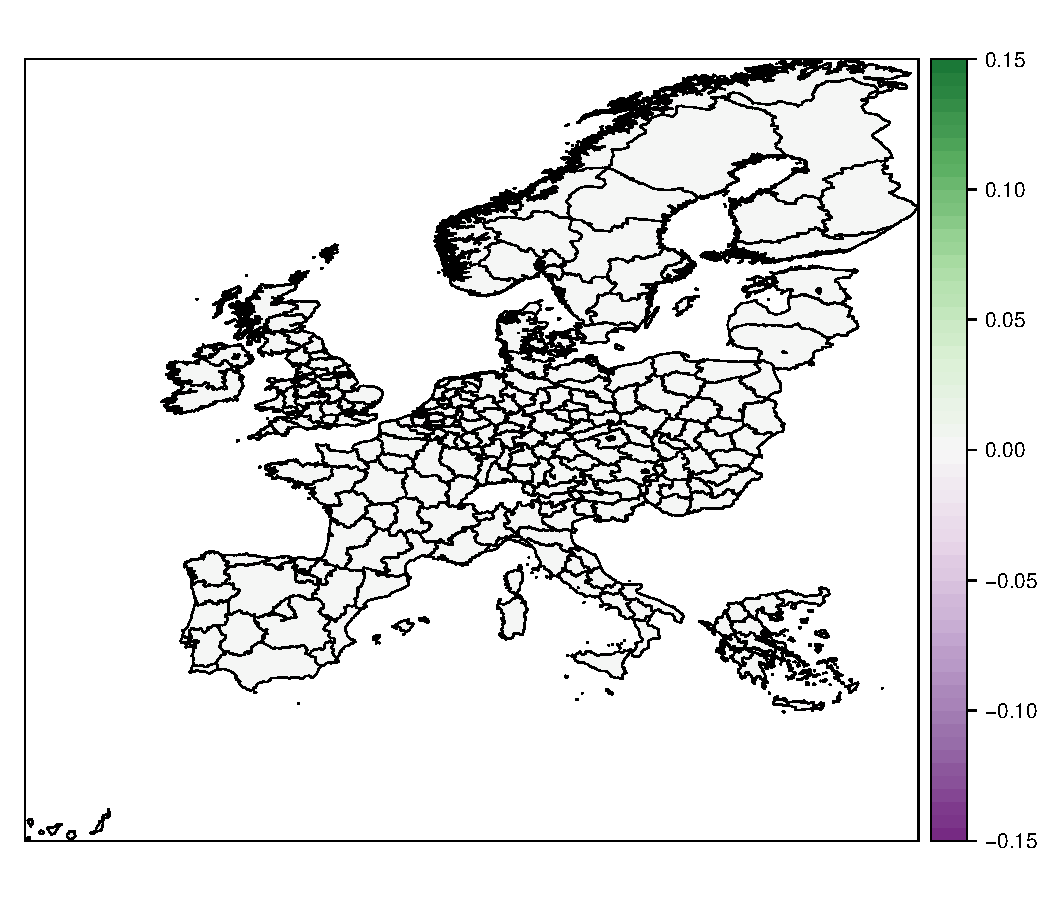
\includegraphics[width=0.5\textwidth]{../Fig/RCAgrhoogopl.pdf} }
	\subfloat[Construction]{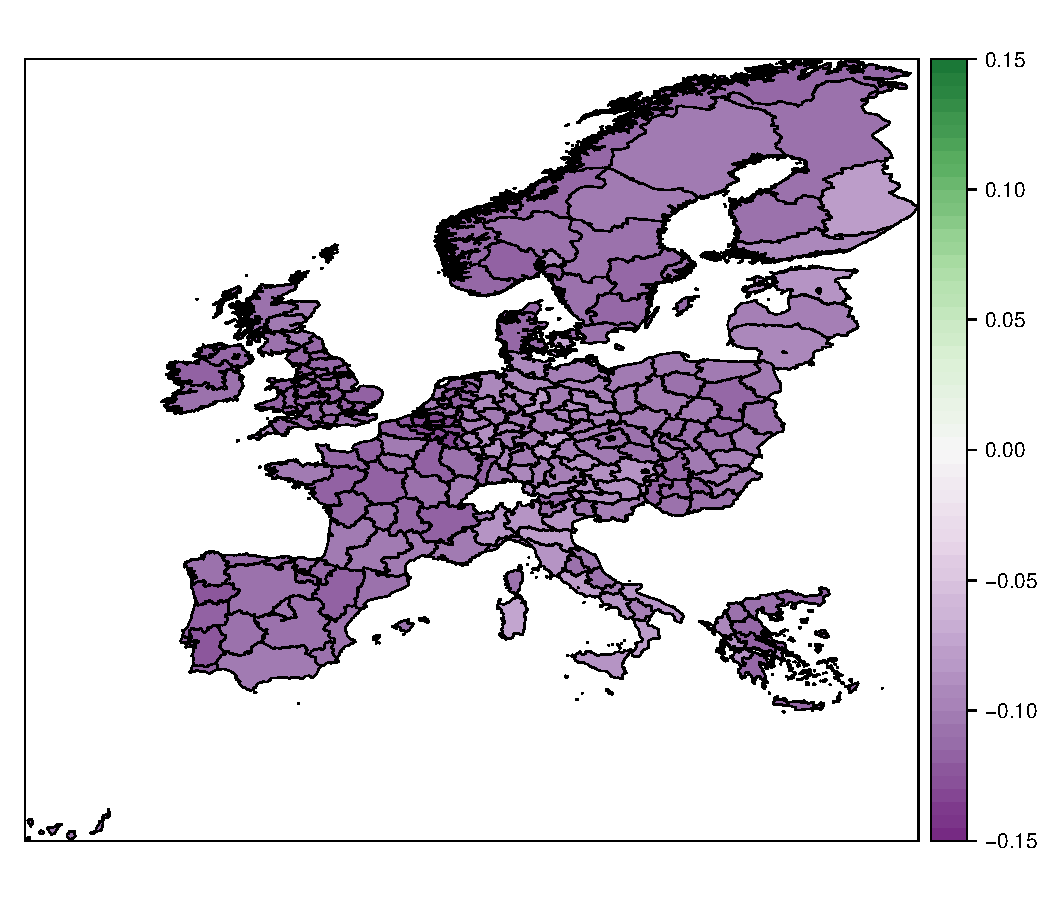
\includegraphics[width=0.5\textwidth]{../Fig/RCConshoogopl.pdf}}\\
	\subfloat[Energy \& Manufacturing]{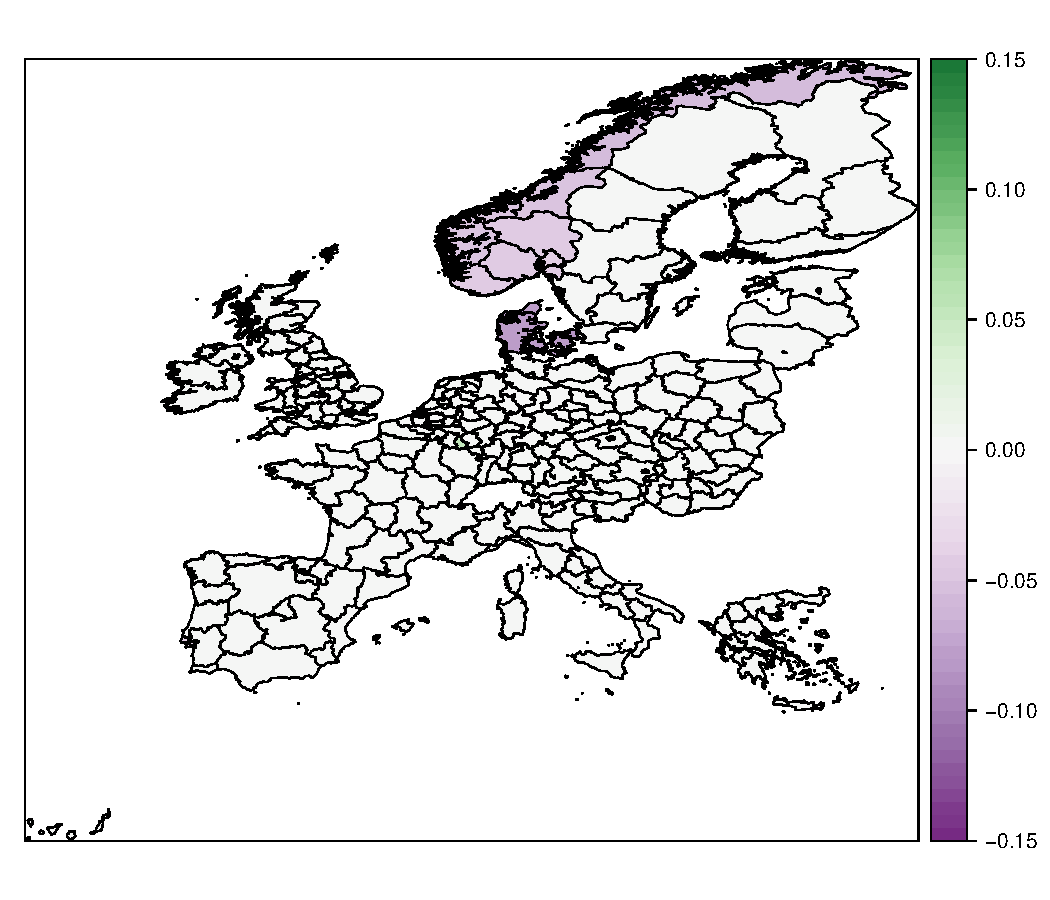
\includegraphics[width=0.5\textwidth]{../Fig/RCEenMhoogopl.pdf} }
	\subfloat[Distribution]{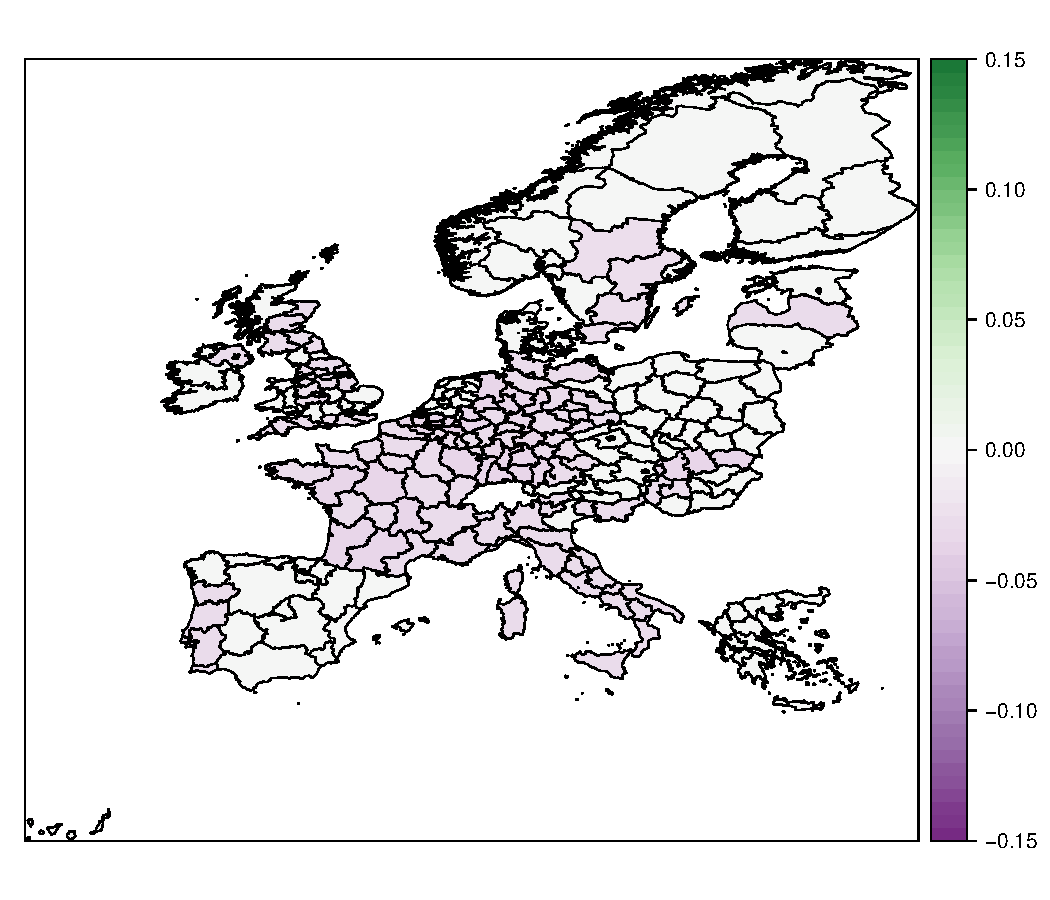
\includegraphics[width=0.5\textwidth]{../Fig/RCDishoogopl.pdf}}\\
	\subfloat[Market services]{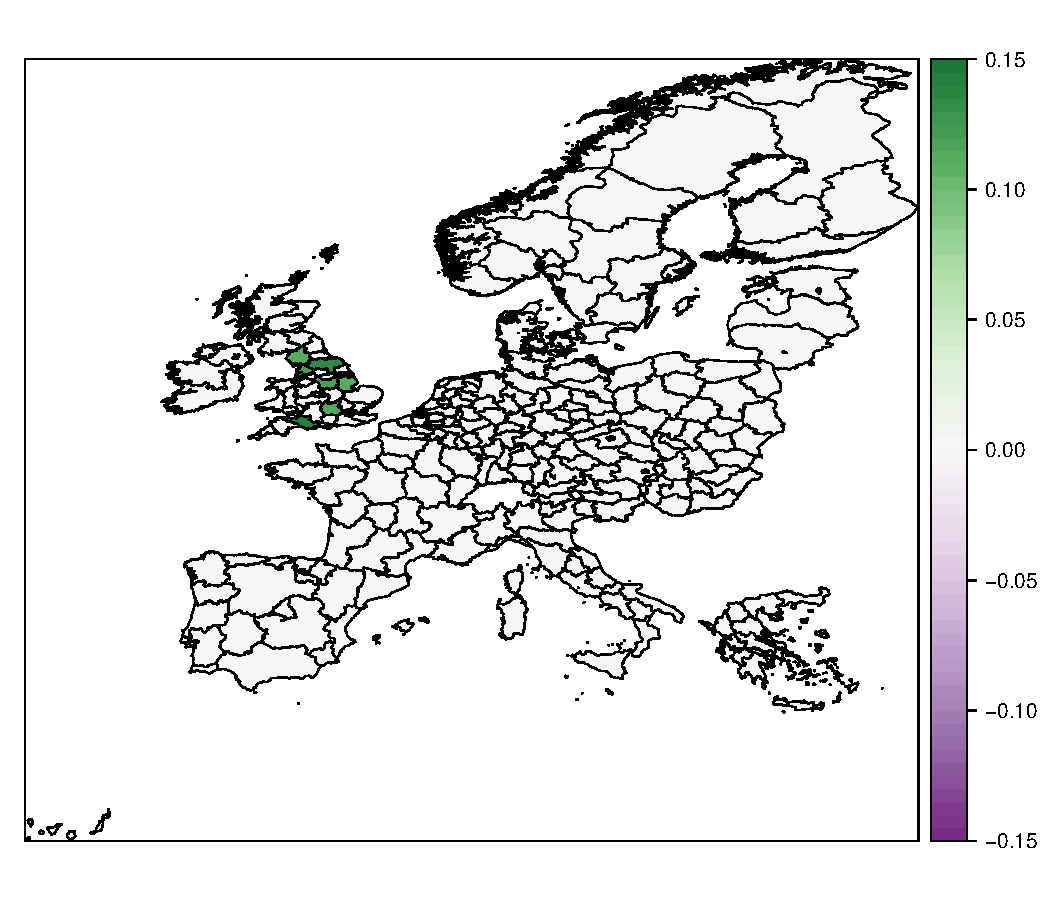
\includegraphics[width=0.5\textwidth]{../Fig/RCServhoogopl.pdf} }
	\subfloat[Non-market services]{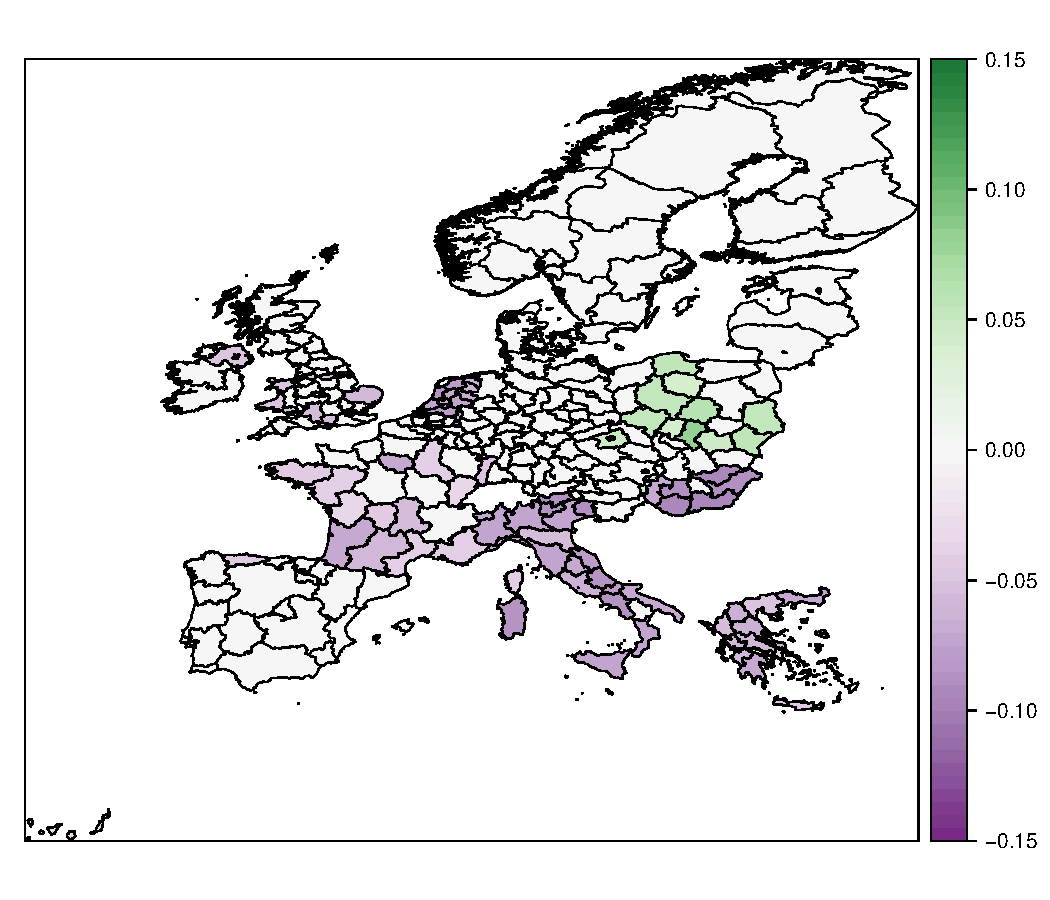
\includegraphics[width=0.5\textwidth]{../Fig/RCNMServhoogopl.pdf}}
	\caption{Impact of highly educated on sectoral growth weighted by the revealed competition network.}
	\label{fig:highedu}
\end{figure}

Figure \ref{fig:highedu} shows clearly that the impact of highly educated on sectoral growth varies over sectors and regions. To start with the impact on agriculture is nowhere statistically significant, where impacts on construction, energy \& manufacturing and distribution are mostly negative, if significant at all, although the size of the impact varies. Interestingly, highly educated positively affects market services only for English regions. The effect on non-market services varies even in sign over regions. Polish regions seem to benefit from the amount of highly educated workers, while especially regions in the Netherlands, France, Italy and Greece, are negatively affected by highly educated workers. Obviously, this is not to say that highly educated workers have a negative affect on the overall performance of a region, but that highly educated workers do not necessarily speed up sectoral growth anymore. Given that in some countries (e.g., The Netherlands) the amount of highly educated workers exceeds more than 50\%, it is to no surprise that this determinant lost its decisive nature.

\begin{figure}
\centering
\subfloat[Agriculture]{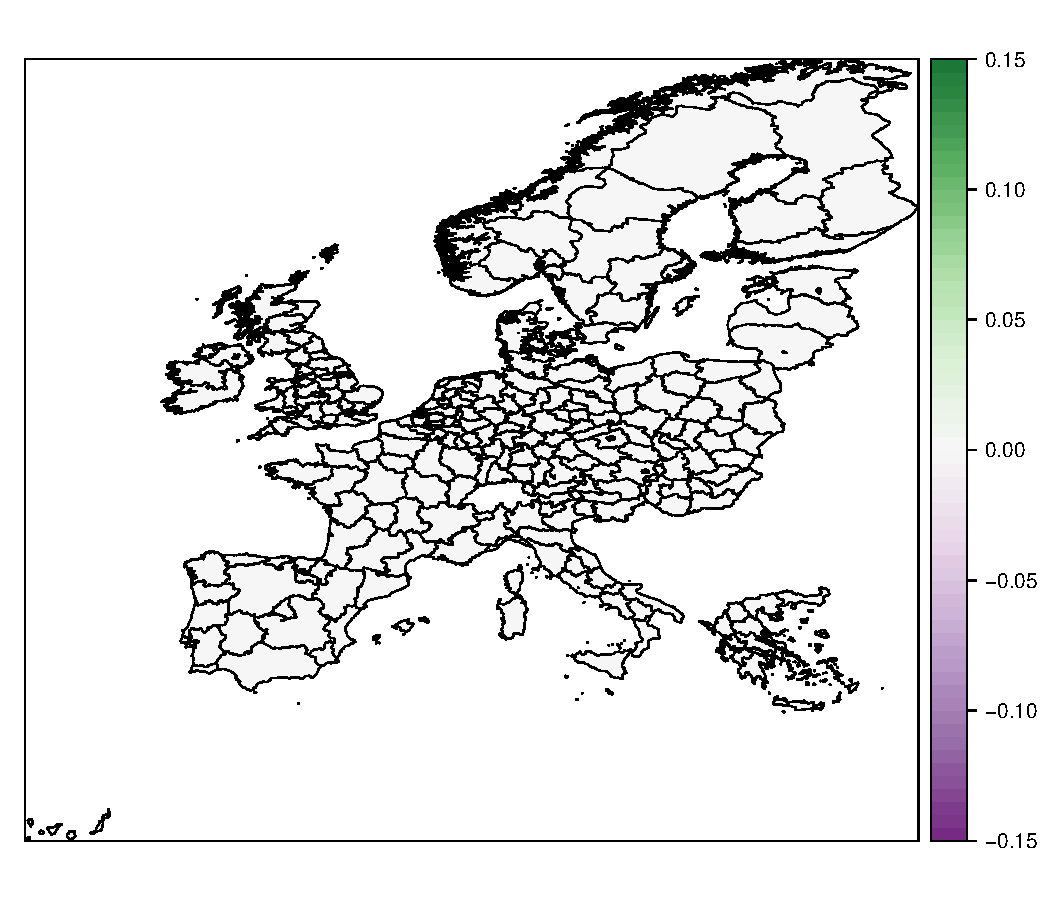
\includegraphics[width=0.5\textwidth]{../Fig/RCAgrBblucht.pdf} }
\subfloat[Construction]{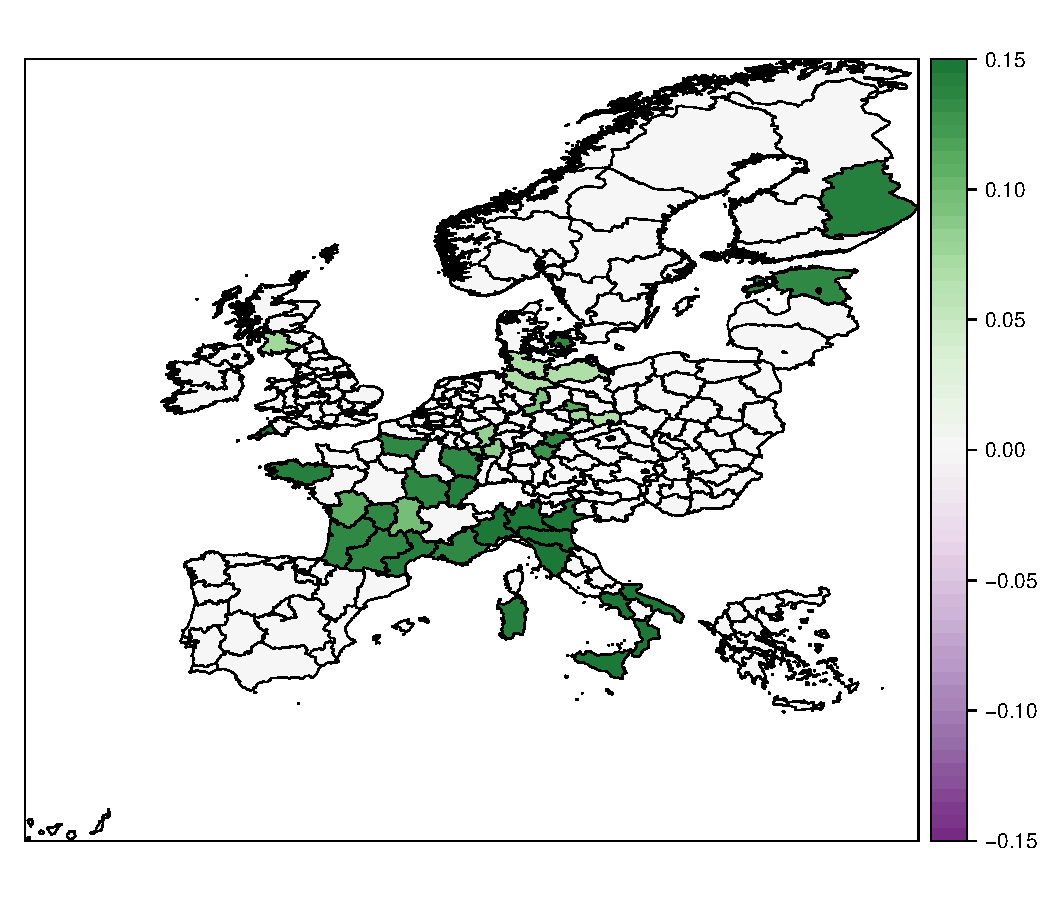
\includegraphics[width=0.5\textwidth]{../Fig/RCConsBblucht.pdf}}\\
\subfloat[Energy \& Manufacturing]{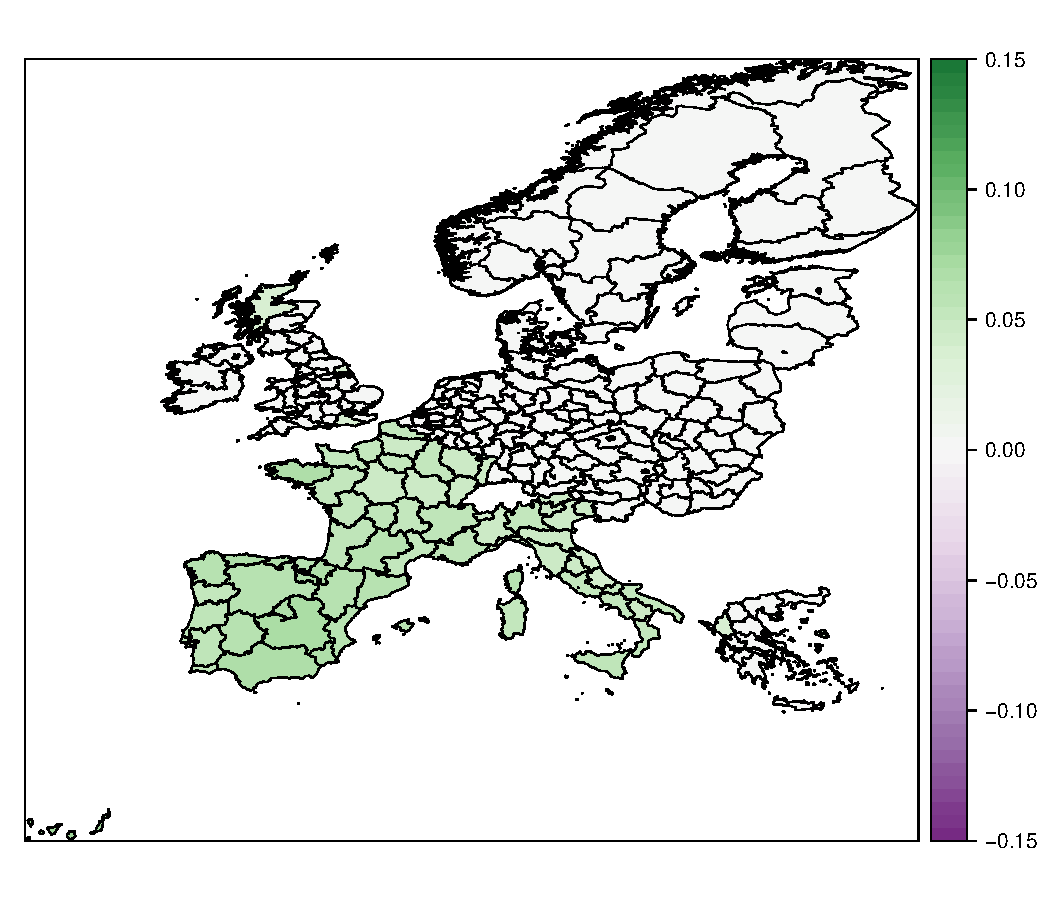
\includegraphics[width=0.5\textwidth]{../Fig/RCEenMBblucht.pdf} }
\subfloat[Distribution]{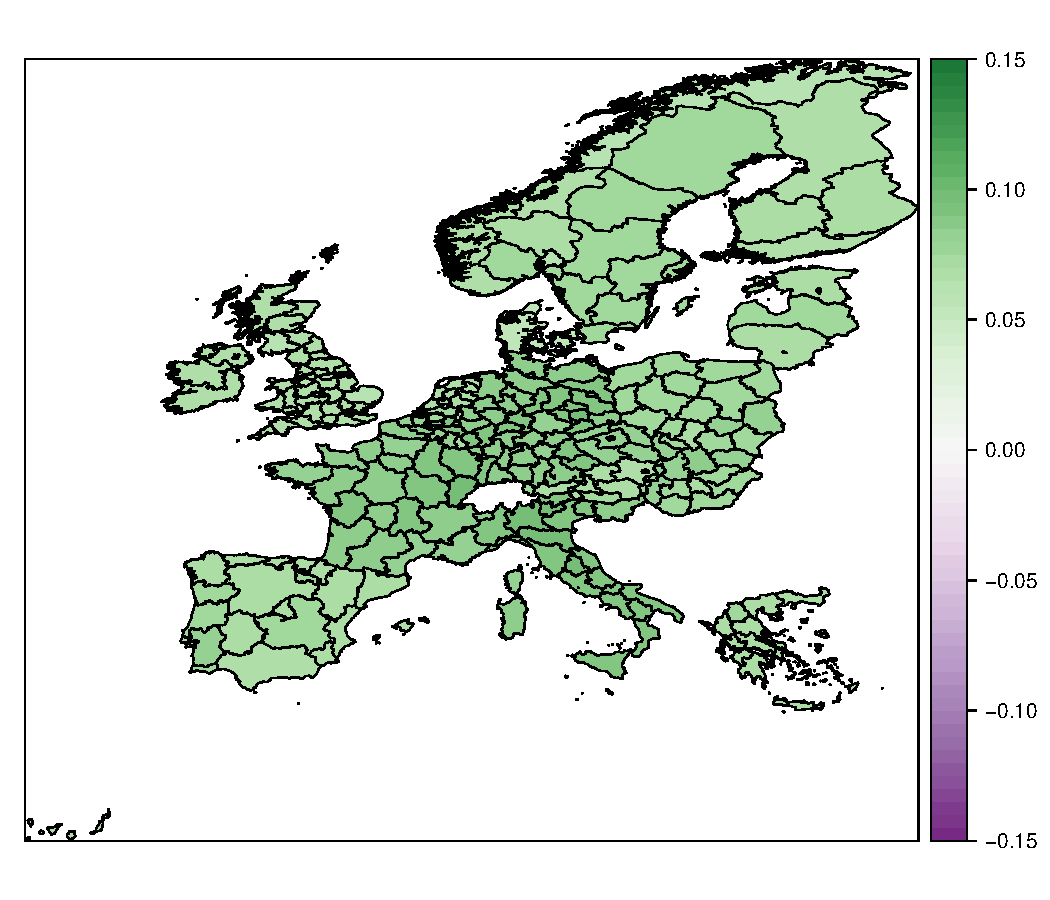
\includegraphics[width=0.5\textwidth]{../Fig/RCDisBblucht.pdf}}\\
\subfloat[Market services]{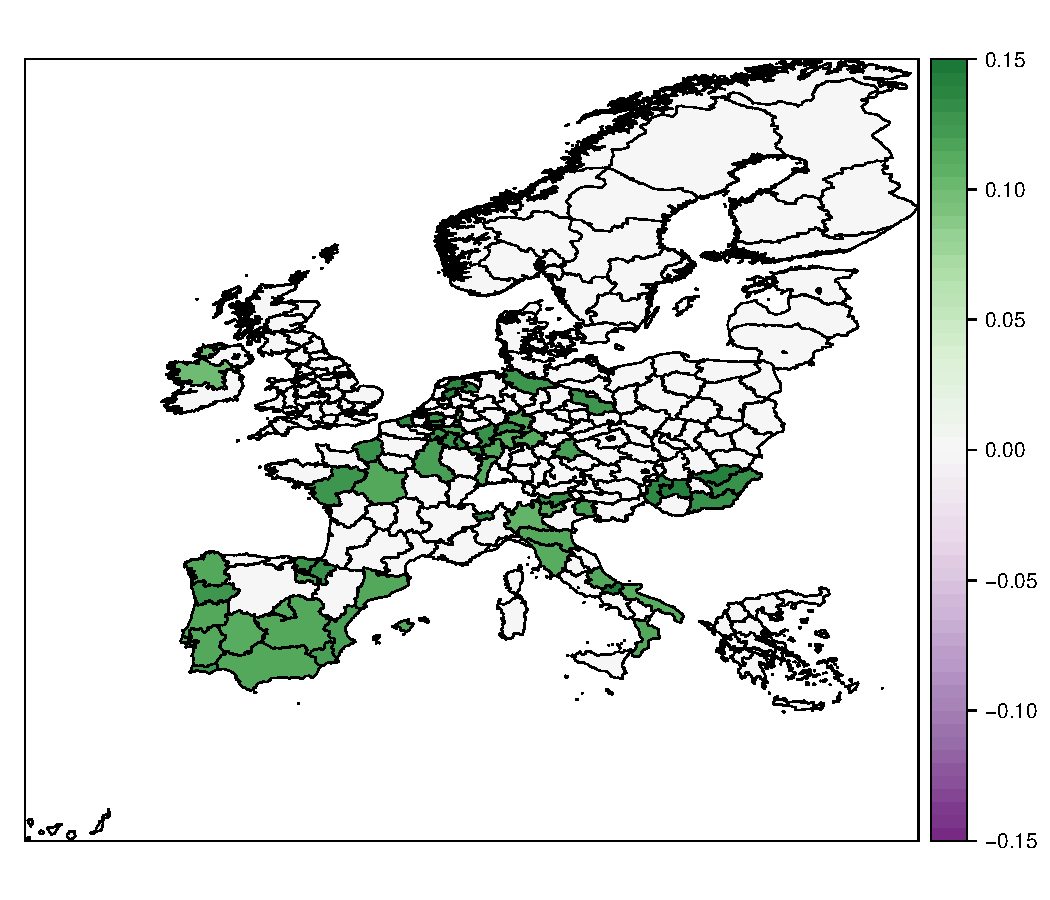
\includegraphics[width=0.5\textwidth]{../Fig/RCServBblucht.pdf} }
\subfloat[Non-market services]{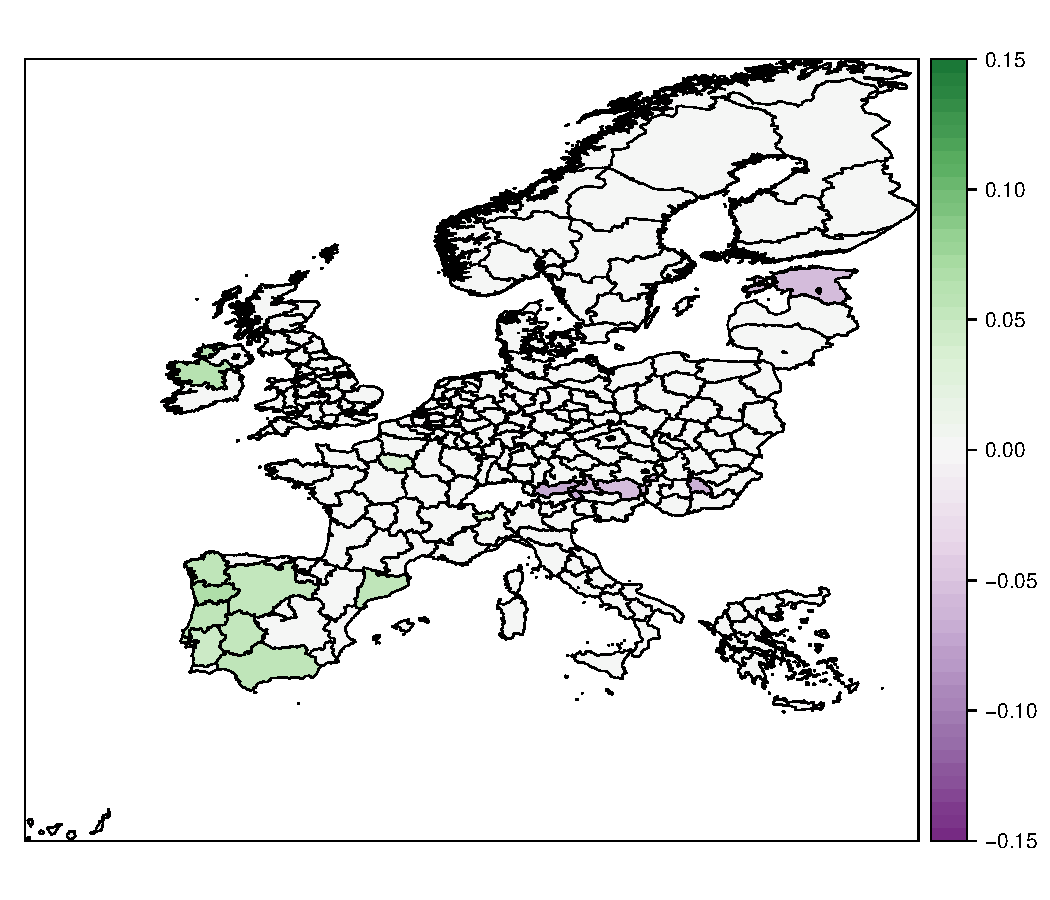
\includegraphics[width=0.5\textwidth]{../Fig/RCNMServBblucht.pdf}}
\caption{Impact of accessibility by air on sectoral growth weighted by the revealed competition network.}
\label{fig:bblucht}
\end{figure}

Figure \ref{fig:bblucht} gives the impact of accessibility by air on sectoral growth, and it plain to see that this impact is mostly positive if statistically significant. Again, this determinant has no effect on the regional structural growth in agriculture. The positive impact on construction can mostly be found in France and Italy, while the positive effect on energy \& manufacturing can mostly as well in Spain. In general, there is an overall positive effect on distribution (which is in contrast with accessibility by road). Moreover, especially the market services benefit largely from accessibility by air in regions scattered all around Europe. Finally, for non-market services there is a heterogenous impact in sign of accessibility by air. Some regional in Spain and Ireland benefit positively, while growth in non-market services in some regions in Eastern Europe is hampered by it. 

Likewise to \ref{fig:highedu} and \ref{fig:bblucht}, maps can be made from the impacts of all other determinants. And all these determinants show a large degree of parameter heterogeneity across sectors and regions, giving additional evidence for the importance of place-based policies. One may wonder, however, how well our revealed competition network performs vis-\`{a}-vis other networks, most notably distance. We therefore re-estimate all parameters using the distance matrix in equation (\ref{eq:weights}) and compare the outcomes of both distance and revealed competion matrices with each other in Table \ref{tab:performance}.\footnote{All maps can be found on this paper's corresponding GitHub repository \url{https://github.com/Thdegraaff/PaperPiRS}.}

\begin{table}[ht]
	\centering
	\caption{Performance in non-parametric regressions of distance and revealed competition matrices}
	\label{tab:performance}
	\begin{tabular*}{\textwidth}{l @{\extracolsep{\fill}} cccc}
		\toprule
		 & \multicolumn{2}{c}{Distance} & \multicolumn{2}{c}{Revealed competition} \\
		 		\cmidrule(r){2-3} \cmidrule(r){4-5} 
		Sector & Adjusted R$^2$ & AIC& Adjusted R$^2$ & AIC  \\
		\midrule
		Agriculture 			& 0.40 & 422.73 	& 0.39 & 428.63\\
		Energy \& Manufacturing & 0.49 & -332.34 	& 0.50 & -345.62 \\ 
		Construction 			& 0.58 & 64.66 		& 0.67 & -0.92 \\
		Distribution 			& 0.56 & -416.80 	& 0.48 	& -358.80\\
		Services 				& 0.13 & 180.83 	& 0.14 	& 179.89\\
		Non-market services 	& 0.55 & -538.15 	& 0.58 & -537.70\\ 
		\bottomrule
	\end{tabular*}
\end{table}

Table \ref{tab:performance} shows the revealed competition networks outperforms the distance matrix in four of the six sectors. Distance only performs better in explaining economic growth in agriculture and distribution. On the one hand this is disappointing because the revealed competition is (\textit{i}) sector specific while distance is not and (\textit{ii}) created especially to explain value added growth. On the other hand, given the fact that distance performs much better in explaining country specific (institutional) effects, this result can be seen as rather strong.\footnote{We tested as well the importance of two other networks, i.e., co-patenting and foreign direct investment networks. These networks did not perform nowhere as good as distance or the revealed competition network.}

\section{Conclusion and discussion}

In this paper we introduced a new theoretical framework to analyze the importance of competitiveness for regional economic growth. 

Our analyses showed that with regard to policy only one size fits one. Although there are general economic processes, they operate in specific (geographical and product) markets that therefore require location specific policies. We found that regional economic performance differs strongly among sectors and regions with a strong geographical and competition component in the location of growth. Regional economic growth does not only take place size-based classes of the largest conurbations or the medium-sized regions, but in regions that have specific characteristics or are embedded in typical networks according. The specific characteristics of these regions depend on, for instance, the sector under investigation. This supports European place-based policy strategies \citep{barca2009agenda,barca2012case} more than place-neutral ones \citep{worldbank2009}.

However, we also find that the effect of these regional characteristics on economic growth is limited and often not significant. This severely limits the possibilities of regional policy makers. In other words, to a large content regional economic development is beyond the control of the (regional) policy maker. And if the policy maker does one want to exert control, mimicking successful regional policies without taking into account the region's specific economic and geographical context is most likely not a recipe for success.

\begin{spacing}{1.2}
	\printbibliography
\end{spacing}
\end{document}
